\newpage

%   (III $\cup$ II) $\cap$ (II' $\cap$ IV)'
\textbf{c)} Analizando paso por paso el segundo inciso \ref{c}, se puede resolver en dos partes \textbf{(III $\cup$ II)} y \textbf{((II' $\cap$ IV)')} para así unir ambos subconjuntos \\

Resolviendo \textbf{(III $\cup$ II)}

\begin{align*}
(III \cup II)  &= \{ a, b, c, d, e, f, g, h, i, j, o, u  \}   \cup \{ h, j, p, q, r, s  \} \\
  &=  \{ a, b, c, d, e, f, g, h, i, j, o, p, q, r, s, u  \}        \\
\end{align*}

Resolviendo \textbf{(II' $\cap$ IV)'}

\begin{align*}
(II' \cap IV)'  &=  (\{ a, b, c, d, e, f, g, i, k, l, m, n, o, t, u, v, w, x, y, z \} \cap \{ f, g, h, j, k, l, m, n, p, q, r, s  \} )' \\
  &=  (\{  f, g, k, l, m, n, \} )' \\
  &= \{ a, b, c, d, e, h, i, j, o, p, q, r, s, t, u, v, w, x, y, z \} \\
\end{align*}

Juntando ambos lados para armar (III $\cup$ II) $\cap$ (II' $\cap$ IV)':

\begin{align*}
(III \cup II) \cap (II' \cap IV)' &= \{ a, b, c, d, e, f, g, h, i, j, o, p, q, r, s, u  \} \cap \{ a, b, c, d, e, h, i, j, o, p, q, r, s, t, u, v, w, x, y, z \}\\
  &= \{ a, b, c, d, e, h, i, j, o, p, q, r, s, u \}
\end{align*}

Por lo tanto el resultado es:

\begin{equation*}
    \boxed{ (III \cup II) \cap (II' \cap IV)' =  \{ a, b, c, d, e, h, i, j, o, p, q, r, s, u \}    }
\end{equation*}



Para obtener el diagrama de Venn, se puede hacer por partes, el lado derecho y lado izquierdo, quedando: \\

\textbf{(III $\cup$ II)}: 

\begin{figure}[htbp]
\centering
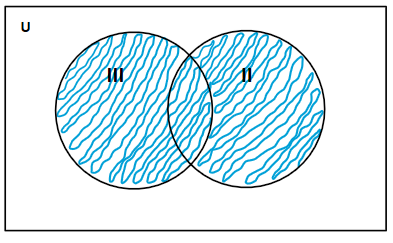
\includegraphics[width=8cm]{c/aa.png}
\caption[]{Diagrama de Venn de (III $\cup$ II)}
\end{figure} 

\newpage

\textbf{(II' $\cap$ IV)'}:

\begin{figure}[htbp]
\centering
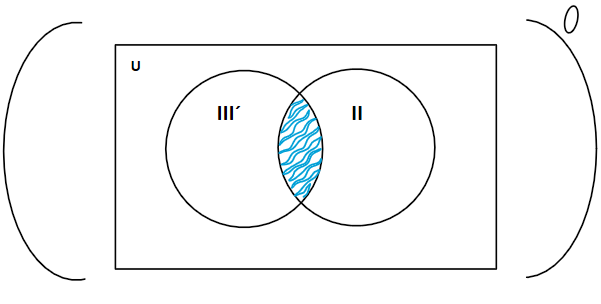
\includegraphics[width=8cm]{c/bb.png}
\caption[]{Diagrama de Venn de (II' $\cap$ IV)'}
\end{figure} 

Sacando el complemento, queda el diagrama

\begin{figure}[htbp]
\centering
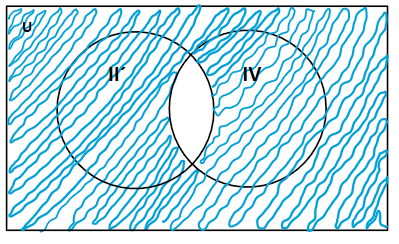
\includegraphics[width=7cm]{c/bbb.png}
\caption[]{Diagrama de Venn de (II' $\cap$ IV)'}
\end{figure} 

Haciendo la intersección de ambos lados para armar (III $\cup$ II) $\cap$ (II' $\cap$ IV)', quedando así el diagrama de Venn:

\begin{figure}[htbp]
\centering
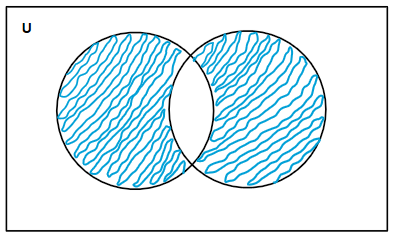
\includegraphics[width=7cm]{c/aabb.png}
\caption[]{Diagrama de Venn de (III $\cup$ II) $\cap$ (II' $\cap$ IV)'}
\end{figure} 
